\documentclass[12pt]{article}

\usepackage[shortlabels]{enumitem}
\usepackage{geometry}
 \geometry{
 a4paper,
 total={170mm,257mm},
 left=20mm,
 top=20mm,
 }
\usepackage{amsmath}
\usepackage{amssymb}
\usepackage{amsfonts}
\usepackage{mathtools}
% \usepackage{hyperref}

\DeclarePairedDelimiter\abs{\lvert}{\rvert}%
\newcommand{\limit}[2]{ \underset{#1\rightarrow #2}{\lim}\, }
\newcommand{\convg}[1]{ \overset{#1}{\rightarrow} }
\newcommand{\var}[1]{ \text{Var}(#1)}
\newcommand{\cov}[2]{ \text{Cov}(#1, #2)}
\newcommand{\expec}[1]{\mathbb{E}[#1]}
\newcommand{\Exp}[1]{ \text{Exponential}(#1)}
\newcommand{\Pois}[1]{ \text{Poisson}(#1)}
\newcommand{\Poisf}[2]{ #2^{#1} \frac{e^{-#2}}{#1!}}

\begin{document}
\title{Homework 1 Responses}
\author{Chris Crabtree}
\date{Sept. 30, 2021}

{
\let\clearpage\relax
\maketitle
}

\begin{enumerate}
    \item
        \stepcounter{section}
\subsection{}
    \prompt{Show that if $\vec{y}\sim EFD(\vec{\theta})$ with EFD being an Exponential Family Distribution, 
then \begin{equation*}\expec{\vec{y}\vert\vec{\theta}} = \partiald{\psi(\vec{\theta})}{\vec{\theta}}\end{equation*}}

For notational convenience I will write $\vec{y\vert\theta}$ as just $\vec{y}$.
\begin{align*}
    1 &= \int_{\vec{y}} h(\vec{y})\exp(\vec{\theta}\tp\vec{y}-\psi(\vec{\theta}))d\vec{y} \tag*{(exp. family dist'n)}\\
    \partiald{}{\vec{\theta}}1 &= \partiald{}{\vec{\theta}}\int_{\vec{y}} h(\vec{y})\exp(\vec{\theta}\tp\vec{y}-\psi(\vec{\theta}))d\vec{y} \\
    0 &= \partiald{}{\vec{\theta}}\exp(-\psi(\vec{\theta}))\int_{\vec{y}} h(\vec{y})\exp(\vec{\theta}\tp\vec{y})d\vec{y}\\
    0 &= \partiald{}{\vec{\theta}}\Big[{\exp(-\psi(\vec{\theta}))}\Big]\int_{\vec{y}} h(\vec{y})\exp(\vec{\theta}\tp\vec{y})d\vec{y}\\
      &{\quad\quad+}{\exp(-\psi(\vec{\theta}))}\partiald{}{\vec{\theta}}\Big[\int_{\vec{y}} h(\vec{y})\exp(\vec{\theta}\tp\vec{y})d\vec{y}\Big]\tag*{(product rule)}\\
    0 &= \partiald{}{\vec{\theta}}\Big[{\exp(-\psi(\vec{\theta}))}\Big]\int_{\vec{y}} h(\vec{y})\exp(\vec{\theta}\tp\vec{y})d\vec{y}\\
      &{\quad\quad+}{\exp(-\psi(\vec{\theta}))}\int_{\vec{y}}\partiald{}{\vec{\theta}}\Big[ h(\vec{y})\exp(\vec{\theta}\tp\vec{y})\Big]d\vec{y}
                                                                                            \tag*{(Leibnitz rule and limits const. w.r.t. $\vec{\theta}$)}\\
    0 &= -\partiald{}{\vec{\theta}}{\Big[\psi(\vec{\theta})\Big]}\exp(-\psi(\vec{\theta}))\int_{\vec{y}} h(\vec{y})\exp(\vec{\theta}\tp\vec{y})d\vec{y}\\
      &{\quad\quad+}{\exp(-\psi(\vec{\theta}))}\int_{\vec{y}}h(\vec{y})\exp(\vec{\theta}\tp\vec{y})\vec{y}d\vec{y}\\
    0 &= -\partiald{}{\vec{\theta}}{\Big[\psi(\vec{\theta})\Big]}\cdot 1 + \expec{\vec{y}}\\
    \expec{\vec{y}} &= \partiald{}{\vec{\theta}}{\Big[\psi(\vec{\theta})\Big]} \\
    \tag*{$\blacksquare$\hspace{5cm}}
\end{align*}


\subsection{}
    % !TEX root = ../*.tex

This has nearly the identical reasoning as in part \ref{Sl_add}, except with a multiplicative factor instead of an additive one.

I will start where the proofs diverge:


Note that,    
\begin{align*}
    \abs{Z_n - z_0} \leq \epsilon &\equiv z_0 - \epsilon \leq Z_n \leq z_0 + \epsilon \\
                               &\Rightarrow \\
    X_n (z_0 - \epsilon) &\leq X_n \cdot Z_n \leq X_n(z_0 + \epsilon), \quad\quad X_n = x \geq 0\\
    X_n (z_0 - \epsilon) &\geq X_n \cdot Z_n \geq X_n(z_0 + \epsilon), \quad\quad X_n = x < 0\\
\end{align*}

Wlog, I will prove the case where $X_n \geq 0$, but the same reasoning applies to the case where $X_n < 0$.
Fixing $\epsilon$, this gives:

\begin{align*}
    \limit{n}{\infty} P(X_n \cdot Z_n \leq a \big\lvert \abs{Z_n - z_0} \leq \epsilon) 
                                                          &\leq \limit{n}{\infty} P(X_n (z_0 - \epsilon) \leq a   )\tag*{(by assumption \ref{asmp2})}\\ 
                                                          &= \limit{n}{\infty} F_{X_n }(a/(z_0- \epsilon))        \tag*{(def. of CDF)}\\
                                                          &= F_{X }(a/(z_0- \epsilon))\tag*{(by assumption \ref{asmp1})}\\  
\end{align*}
Note that we do not need to consider the case when $z_0 - \epsilon = 0$.
This is because $\epsilon$ can be arbitrarily small by the definition of convergence in probability.
We can therefore always assume $z_0 - \epsilon > 0$ since we can just limit our consideration to values of $\epsilon$ smaller than $z_0$.

When combined with the other inequality, this gives:
\begin{equation*}
    F_{X}(a /(z_0 + \epsilon ))   \leq  \limit{n}{\infty} P(X_n + Z_n \leq a) \leq F_{X}(a /(z_0 - \epsilon ))\\
\end{equation*}

The rest of the proof is exactly the same as in part \ref{Sl_add}, so I will omit it.


    \item 
        \section{}

We use the following stochastic process as our data generation model for the time dependent variable $y_t$ in an arbitrary time step $t\in[1,T]$.
Note that, except for the $y_t$'s, all of the following are random variables generated by parametric distributions defined by our model.
The stochastic process is modelled as follows:
\begin{align}
    \nonumber&\mathbf{z}_{1} =  \mathbf{s}_0\\
    \nonumber&y_1 =  \mathbf{x}_1 {}^\intercal  \mathbf{z}_1\\
    \nonumber&\mathbf{z}_{2} =  \mathbf{Z}_2^*{}\cdot \mathbf{z}_1 \\
    \nonumber&y_2 = \mathbf{x}_2 {}^\intercal \mathbf{z}_2 \\
    \nonumber&\mathbf{z}_{3} =  \mathbf{Z}_3^*{}\cdot \mathbf{z}_2 \\
    \nonumber&\quad \vdots \\
    \nonumber&\mathbf{z}_{t-1} =  \mathbf{Z}^*_{t-1}{}\cdot \mathbf{z}_{t-2} \\
    \label{q2:model_transition1}
    &y_{t-1} =  \mathbf{x}_{t-1} {}^\intercal \mathbf{z}_{t-1} \\
    \label{q2:model_transition2}
    &\mathbf{z}_{t} =  \mathbf{Z}^*_{t}{}\cdot \mathbf{z}_{t-1} \\
    &y_{t} = \mathbf{x}_{t} {}^\intercal \mathbf{z}_t
    \label{q2:model}
\end{align}
With $\mathbf{z}_t$  and the columns of $\mathbf{Z}^*_t$, $t \in [1, T]$, being random standard basis vectors in $\mathbb{R}^K$.
As such, I will use $z_t$ to denote the index of the non-zero entry in $\mathbf{z}_t$ and likewise $\mathbf{z}^*_{tj}{}^\intercal$ to denote the $j^{th}$ column of $\mathbf{Z}_t^*$.

I will also use the notation $\mathbf{z}_{1:t} \in \mathbb{R}^{K\times t}$ to refer to the sequence of $\mathbf{z}_t$ vectors chosen on the left side of the equalities in the above generation.
$\mathbf{Z}_t^* \in \mathbb{R}^{K\times K}$ is akin to a set of candidate $\mathbf{z}_t$'s.
From the above sequence, it should be clear that $\mathbf{z}_{t}$ determines both $\mathbf{y}_{t}$ and $\mathbf{z}_{t+1}$.
$\mathbf{z}_{t}$ is effectively the $z_{t-1}{}^{th}$ column of $\mathbf{Z}^*_{t}$.
$\mathbf{a}_0$ and $\mathbf{Z}^*_{t}$ are distributed as follows:
\begin{align}
    &\mathbf{s}_0 \sim \text{Multi}(1, \boldsymbol{\pi}_0), \boldsymbol{\pi}_0 \in \mathbb{R}^K\\
    &\boldsymbol{\pi}_0 \sim \text{Dir}(1/K, 1/K, \cdots, 1/K)\\
    \label{q2:zt+1_dist}
      &\mathbf{Z}_{t}^* = 
    \begin{bmatrix}\mathbf{z}_{t1}^*&
        \mathbf{z}_{t2}^*&
        \cdots & 
        \mathbf{z}_{tK}^*
            \end{bmatrix} 
    \sim 
    \begin{bmatrix}
        \text{Multi}(1, \boldsymbol{\pi}_{1})&
        \text{Multi}(1, \boldsymbol{\pi}_{2})& 
        \vdots&
        \text{Multi}(1, \boldsymbol{\pi}_{K})
    \end{bmatrix},\;
    \boldsymbol{\pi}_i\in \mathbb{R}^K\\
    &\mathbf{P} = 
    \begin{bmatrix}
        \pi_{11} & \pi_{12} & \cdots &\pi_{1K}\\
        \pi_{21} & \pi_{22} & \cdots &\pi_{2K}\\
        \vdots & &\cdots&\vdots \\ 
\pi_{K1} & \pi_{K2} & \cdots &\pi_{KK}\\
    \end{bmatrix} 
    =
    \begin{bmatrix}
        \boldsymbol{\pi}_1{}^\intercal\\
        \boldsymbol{\pi}_2{}^\intercal\\
        \vdots \\ 
        \boldsymbol{\pi}_K{}^\intercal
    \end{bmatrix} 
      \distiid \text{Dir}(1/K, 1/K, \cdots , 1/K)\\
\end{align}

$\mathbf{x}_t$ is defined as follows with $\mathbf{P}$ having the same definition as above:
\begin{align}
    &\mathbf{x}_t = 
    \begin{bmatrix}
        x_{t1} \\
        x_{t2}\\
        \vdots \\
        x_{tK} \\
    \end{bmatrix}
    \distiid
    MVN(\boldsymbol{\mu}, \boldsymbol{\sigma}^2 {}^\intercal \mathbf{I})=
    % \begin{bmatrix}
    %     \mathbf{z}^*_{t1}{}^\intercal\\
    %     \mathbf{z}^*_{t2}{}^\intercal\\
    %     \vdots\\
    %     \mathbf{z}^*_{tK}{}^\intercal\\
    % \end{bmatrix} \cdot 
    \begin{bmatrix}
        \mathcal{N}(\mu_1, \sigma^2_1)\\
        \mathcal{N}(\mu_2, \sigma^2_2)\\
        \vdots\\
        \mathcal{N}(\mu_K, \sigma^2_K)\\
    \end{bmatrix}\\
    &\mu_j \distiid \text{Normal-Inv-Gamma}(\mu_0, \sigma^2_0/\kappa_0, \nu_0, \sigma^2_0)\\
\end{align}



We are interested in the posterior.
I will denote it as:

\begin{align}
    p(\boldsymbol{\mu}, \boldsymbol{\sigma}^2, \mathbf{P}|y_{1:t}, \mu_0, \sigma_0, \alpha_0, \beta_0)  
\end{align}
Bayes theorem then gives us:
\begin{align}
    p(\boldsymbol{\mu}, \boldsymbol{\sigma}^2, \mathbf{P}|y_{1:t}, \mu_0, \sigma_0, \alpha_0, \beta_0) &=
    \frac{p(y_{1:t} |\boldsymbol{\mu}, \boldsymbol{\sigma}^2, \mathbf{P}, \mu_0, \sigma_0, \alpha_0, \beta_0)
    p_0( \boldsymbol{\mu}, \boldsymbol{\sigma}^2, \mathbf{P}| \mu_0, \sigma_0, \alpha_0, \beta_0)}
    {\int_{\boldsymbol{\mu}, \boldsymbol{\sigma}^2, \mathbf{P}} p(y_{1:t} |\boldsymbol{\mu}, \boldsymbol{\sigma}^2, \mathbf{P}, \mu_0, \sigma_0, \alpha_0, \beta_0)
    p_0( \boldsymbol{\mu}, \boldsymbol{\sigma}^2, \mathbf{P}| \mu_0, \sigma_0, \alpha_0, \beta_0)}\\[10pt]
    &\propto p(y_{1:t} |\boldsymbol{\mu}, \boldsymbol{\sigma}^2, \mathbf{P}, \mu_0, \sigma_0, \alpha_0, \beta_0)
    p_0( \boldsymbol{\mu}, \boldsymbol{\sigma}^2, \mathbf{P}| \mu_0, \sigma_0, \alpha_0, \beta_0)
\end{align}

First I will concentrate on the likelihood.
Since we use the HMM model for time dependency, the likelihood can be decomposed simply.
I will omit the priors to simplify notation (they are there, but won't be involved in any likelihood calculations).
The likelihood is now:
\begin{align}
    p(y_{1:T} |\boldsymbol{\mu}, \boldsymbol{\sigma}^2, \mathbf{P}, \boldsymbol{\pi_0})
                       &=\nonumber
                        \sum_{\mathbf{z}_{1:T}} p(y_{1:T} |\mathbf{z}_{1:T}, \boldsymbol{\mu}, \boldsymbol{\sigma}^2, \mathbf{P}, \boldsymbol{\pi_0})
                        p(\mathbf{z}_{1:T}|\boldsymbol{\mu}, \boldsymbol{\sigma}^2, \mathbf{P}, \boldsymbol{\pi_0})\\
                       &=\nonumber
                       \sum_{j=1}^K p(y_T |z_T=j, \boldsymbol{\mu}, \boldsymbol{\sigma}^2)p(z_T=j| z_{(T-1)}, \mathbf{P})\times\\
                         \nonumber&{\qquad\qquad\qquad\qquad}  \sum_{\mathbf{z}_{1:(T-1)}}p(y_{1:(T-1)} | z_{1:(T-1)}, \boldsymbol{\mu}, \boldsymbol{\sigma}^2) 
                        \tag*{(HMM assumption)}\\
                       &=\nonumber
                       \sum_{j=1}^K p(y_T |z_T=j, \boldsymbol{\mu}, \boldsymbol{\sigma}^2)\times\\
                      \nonumber &{\qquad\qquad} \sum_{i=1}^Kp(z_T=j| z_{(T-1)}=i, \mathbf{P}) \sum_{\mathbf{z}_{1:(T-1)}}p(y_{1:(T-1)} | z_{1:(T-1)}, \boldsymbol{\mu}, \boldsymbol{\sigma}^2, \mathbf{P}, \boldsymbol{\pi_0})\\
                       &=\nonumber
                       \sum_{j=1}^K p(\mathbf{x}^\intercal\mathbf{z}_T |z_T=j, \boldsymbol{\mu}, \boldsymbol{\sigma}^2)\times\\
                       \label{q2:likelihood_w_zs}
                       &{\qquad} \sum_{i=1}^Kp(\mathbf{z}_{T}=\mathbf{Z}^{*}_T\cdot \mathbf{z}_{T-1} \Rightarrow z_{T} = j| z_{(T-1)}=i, \mathbf{P}) \sum_{\mathbf{z}_{1:(T-1)}}p(y_{1:(T-1)} | z_{1:(T-1)}, \boldsymbol{\mu}, \boldsymbol{\sigma}^2, \mathbf{P}, \boldsymbol{\pi_0})\\
                       &=
                       \label{q2:orig_likelihood}
                       \sum_{j=1}^K \mathcal{N}(y_t|\mu_i, \sigma_i^2)\times\sum_{i=1}^K \boldsymbol{\pi}_{ij} 
                         \sum_{\mathbf{z}_{1:(T-1)}}p(y_{1:(T-1)} | z_{1:(T-1)}, \boldsymbol{\mu}, \boldsymbol{\sigma}^2, \mathbf{P}, \boldsymbol{\pi_0})\\
\end{align}
This summation is effectively over every possible combination of $z_t$s through time.
A recursive definition is used here to allow for easier computation. 
Since the last factor is independent of both the $j$ indexer we only need to store the $K$ values for the $T-1$ time step.
Note that the notation $\mathcal{N}(y_t|\mu_{z_t}, \sigma_{z_t}^2)$ refers to the density of $y_t$ using the Normal distribution given those parameters.
This is for clarification purposes. 
We can use the density here because the posterior we are calculating is acually a density despite the $p(\cdots)$ notation.



\begin{align}
    &p_0( \boldsymbol{\mu}, \boldsymbol{\sigma}^2, \mathbf{P}| \mu_0, \sigma_0, \alpha_0, \beta_0) \\
    &{\qquad\qquad}\propto \prod_{j=1}^K \text{Normal-Inv-Gamma}((\mu_j, \sigma^2_j)|\mu_0, \sigma^2_0/\kappa_0, \nu_0, \sigma^2_0)\times\prod_{i=1}^K\text{Dir}(\boldsymbol{\pi}_i|1/K, 1/K, \cdots, 1/K)\\
\end{align}
I separated the product for clarity.
Each element of the $K$ elements of  $\boldsymbol{\mu}$ and $\boldsymbol{\sigma}^2$ were generated once and likewise each $\boldsymbol{\pi_i}\in \mathbf{P}$ was generated once.
With this we can finally write the posterior as:
\begin{align}
    &p(\boldsymbol{\mu}, \boldsymbol{\sigma}^2, \mathbf{P}|y_{1:t}, \mu_0, \sigma_0, \alpha_0, \beta_0) \\
    &{\qquad\qquad\qquad\propto}\\
                      &p(y_{1:t} |\boldsymbol{\mu}, \boldsymbol{\sigma}^2, \mathbf{P}, \mu_0, \sigma_0, \alpha_0, \beta_0)
    \times p_0( \boldsymbol{\mu}, \boldsymbol{\sigma}^2, \mathbf{P}| \mu_0, \sigma_0, \alpha_0, \beta_0)\\
    &{\qquad\qquad\qquad=}\\
    &p(y_{1:t} |z_{1:t}, \boldsymbol{\mu}, \boldsymbol{\sigma}^2, \mathbf{P}, \mu_0, \sigma_0, \alpha_0, \beta_0)
        p( z_{1:t}| \boldsymbol{\mu}, \boldsymbol{\sigma}^2, \mathbf{P}, \mu_0, \sigma_0, \alpha_0, \beta_0)
    \times p_0( \boldsymbol{\mu}, \boldsymbol{\sigma}^2, \mathbf{P}| \mu_0, \sigma_0, \alpha_0, \beta_0)\\
    &{\qquad\qquad\qquad}\propto\\
    \label{q2:prop_posterior}
    &\sum_{j=1}^K \mathcal{N}(y_t|\mu_i, \sigma_i^2)\times\sum_{i=1}^K \boldsymbol{\pi}_{ij} 
         \sum_{\mathbf{z}_{1:(T-1)}}p(y_{1:(T-1)} | z_{1:(T-1)}, \boldsymbol{\mu}, \boldsymbol{\sigma}^2, \mathbf{P}, \boldsymbol{\pi_0})\\
    &{\qquad\qquad\qquad}\times\\
      &\prod_{j=1}^K \text{Normal-Inv-Gamma}((\mu_j, \sigma^2_j)|\mu_0, \sigma^2_0/\kappa_0, \nu_0, \sigma^2_0)\times\prod_{i=1}^K\text{Dir}(\boldsymbol{\pi}_i|1/K, 1/K, \cdots, 1/K)\\
\end{align}

Now we need the conditionals of $\boldsymbol{\mu}$, $\boldsymbol{\sigma^2}$, and $\boldsymbol{P}$ to be able to use Gibbs sampling.
We must include the $\mathbf{z}_{1:t}$'s in our conditioning to make the computation tractable.
We start with the $\mathbf{z}_{1:t}$'s.
We can ignore the prior since the $\mathbf{z}_{1:t}$'s do not appear there.
Looking at Eq. \ref{q2:likelihood_w_zs} it should be clear that each $\mathbf{z}_t$ can be sampled iteratively using the recursive definition provided.
Each $\mathbf{z}_t$ is involved in emitting $y_t$ and in choosing $\mathbf{z}_{t+1}$. 
I used the Forward algorithm to do this.
One note is that I computed everything in log-space for numerical stability rather than the telescoping normalization.


Now for $\boldsymbol{\pi}_j^\intercal \in \mathbf{P}$'s. 
For this we must think about what affects each $\boldsymbol{\pi}_j^\intercal$ in the posterior. 
The prior must be included, clearly, but the likelihood needs special attention.
In particular, in Eq. \ref{q2:likelihood_w_zs} we can notice that a $\pi_{:j}$ only appears in Eq. \ref{q2:orig_likelihood} when it is chosen by $\mathbf{z}_{t+1}$.
% $\boldsymbol{\pi}_j$ is only involved in if $z_{t-1} = j$.
% $z_{t-1}$ could be from any column $\mathbf{z}^*_{(t-1)i} \in \mathbf{Z^*_t}$. 
Since the $\mathbf{z}_{1:T}$s are given, we can simply count the number of $z_{t-1} = i$ and $z_t =j$ for all $t\in[1, T]$ and $i\in [1,K]$.
Each time that occurs a $\pi_{ij}$ will appear in the likelihood.
Therefore we have: 
\begin{align}
    p(\boldsymbol{\pi}_j|-) &\propto 
    \prod_{t=1}^T \pi_{ij}^{\mathbbm{1}(z_{t-1} = i \land z_t = j)} \text{Dir}(\boldsymbol{\pi}_j|1/K, 1/K, \cdots, 1/K)
     % p(\boldsymbol{\pi}_i|-) &= \frac{\prod_{t\in \mathcal{Z}_j}p(z_t = i| \mathbf{P}, \boldsymbol{\pi}_0) \text{Dir}(\boldsymbol{\pi_i}|1/K, 1/K, \cdots, 1/K)}
     %                        {\sum_{j=1}^K\prod_{t\in \mathcal{Z}_j}p(z_t = i| \mathbf{P}, \boldsymbol{\pi}_0) \text{Dir}(\boldsymbol{\pi_i}|1/K, 1/K, \cdots, 1/K)}\\
\end{align}

The $\mathbf{\mu}$ and $\mathbf{\sigma}^2$ parameters are drawn from a Normal-Inv-Gamma distribution since it is conjugate to our likelihood with unknown $\mu$s and $\sigma^2$s. 
I used the parameter updates described in module 5 slide 6. 
The only difference is that for each component $j$, I only incorporate the datapoints from time steps where $z_t = j$.

Figure \ref{fig:K_components} shows the results of fitting $K$ component mixtures.
I did not have time to complete the other plots, but they should be easy compared to the actual algorithm.
For the stationary distribution I computed the eigendecomposition of the $\mathbf{P}$ matrix and found the eigenvector corresponding the eigenvalue of $1$.
Then I just normalized that eigenvector. 


\begin{figure}
     \centering
     \begin{subfigure}[b]{0.3\textwidth}
         \centering
         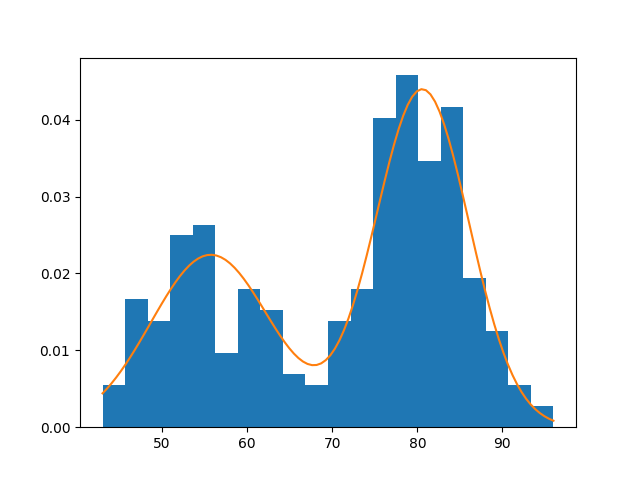
\includegraphics[width=\textwidth]{../code/q2/data_hist_k2.png}
         \caption{K=2}
         \label{fig:k=2}
     \end{subfigure}
     \hfill
     \begin{subfigure}[b]{0.3\textwidth}
         \centering
         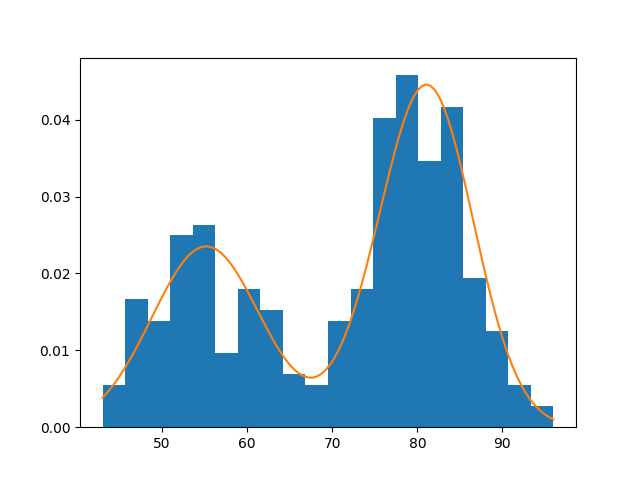
\includegraphics[width=\textwidth]{../code/q2/data_hist_k3.png}
         \caption{K=3}
         \label{fig:k=3}
     \end{subfigure}
     \hfill
     \hfill
     \begin{subfigure}[b]{0.3\textwidth}
         \centering
         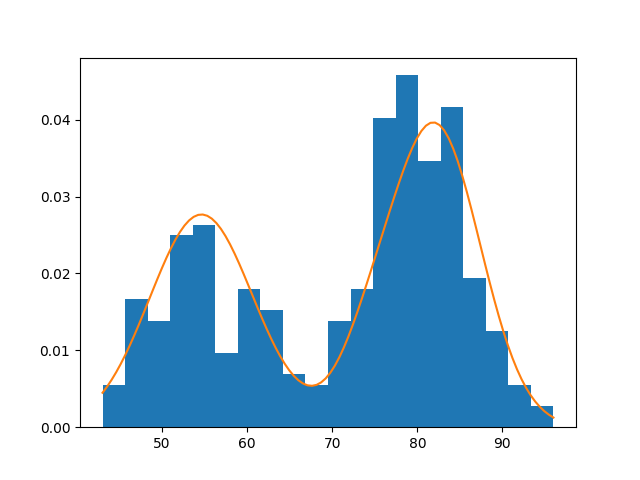
\includegraphics[width=\textwidth]{../code/q2/data_hist_k4.png}
         \caption{K=4}
         \label{fig:k=4}
     \end{subfigure}
     \hfill
     \begin{subfigure}[b]{0.3\textwidth}
         \centering
         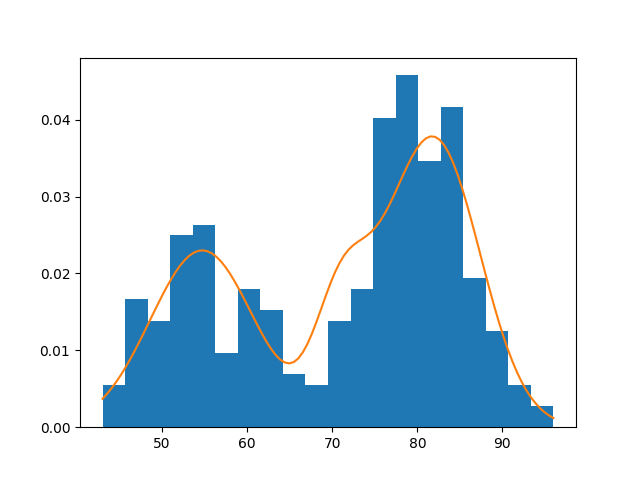
\includegraphics[width=\textwidth]{../code/q2/data_hist_k5.png}
         \caption{K=5}
         \label{fig:k=5}
     \end{subfigure}
     % \hfill
     % \begin{subfigure}[b]{0.3\textwidth}
     %     \centering
     %     \includegraphics[width=\textwidth]{../code/regular_loc_scale_plots/galaxies_hist_k_9.png}
     %     \caption{K=}
     %     \label{fig:Reg_loc_scale}
     % \end{subfigure}
        \caption{Estimated density using Gibbs sampled $\mu$s and $\sigma^2$'s and the stationary distribution from the largest eigenvector.
        I did not have time to figure out how python can plot the credible intervals, although I have all samples so it shouldn't be hard.}
        \label{fig:K_components}
\end{figure}



    \item
        \stepcounter{section}
\subsection{}
    Plots are given in figure \ref{fig:Reg_loc_only}. 
I used the log-likelihood function as my stopping criteria.
For the these non-stochastic experiments I stopped iterating when the improvement in the log-likelihood was less than .001.




\begin{figure}
     \centering
     \begin{subfigure}[b]{0.3\textwidth}
         \centering
         \includegraphics[width=\textwidth]{../code/regular_loc_only_plots/galaxies_hist_k_4.png}
         \caption{K=4}
         \label{fig:Reg_loc_only4}
     \end{subfigure}
     \hfill
     \begin{subfigure}[b]{0.3\textwidth}
         \centering
         \includegraphics[width=\textwidth]{../code/regular_loc_only_plots/galaxies_hist_k_6.png}
         \caption{K=6}
         \label{fig:Reg_loc_only6}
     \end{subfigure}
     \hfill
     \begin{subfigure}[b]{0.3\textwidth}
         \centering
         \includegraphics[width=\textwidth]{../code/regular_loc_only_plots/galaxies_hist_k_8.png}
         \caption{K=8}
         \label{fig:Reg_loc_only8}
     \end{subfigure}
     \begin{subfigure}[b]{0.3\textwidth}
         \centering
         \includegraphics[width=\textwidth]{../code/regular_loc_only_plots/galaxies_hist_k_11.png}
         \caption{K=11}
         \label{fig:Reg_loc_only11}
     \end{subfigure}
     \hfill
     \begin{subfigure}[b]{0.3\textwidth}
         \centering
         \includegraphics[width=\textwidth]{../code/regular_loc_only_plots/galaxies_hist_k_15.png}
         \caption{K=15}
         \label{fig:Reg_loc_only15}
     \end{subfigure}
     \hfill
     \begin{subfigure}[b]{0.3\textwidth}
         \centering
         \includegraphics[width=\textwidth]{../code/regular_loc_only_plots/galaxies_hist_k_20.png}
         \caption{K=20}
         \label{fig:Reg_loc_only20}
     \end{subfigure}
        \caption{Non-Stochastic 1-D Location Mixtures}
        \label{fig:Reg_loc_only}
\end{figure}

\subsection{}
    Tabulated AIC and BIC scored below:
\vspace{4mm}

\begin{tabular}{lllr}
\toprule
{} &     aic &     bic &  iters \\
k  &         &         &        \\
\midrule
4  &  433.4* &  455.1* &     88 \\
6  &   450.7 &   482.0 &     40 \\
8  &   449.4 &   490.4 &    267 \\
11 &   440.0 &   495.4 &    173 \\
15 &   448.6 &   523.2 &    179 \\
20 &   468.7 &   567.4 &    476 \\
\bottomrule
\end{tabular}

\vspace{4mm}
\noindent Best values of each are marked with a *.


\subsection{}
    Plots for the location-scale models are given in figure \ref{fig:Reg_loc_scale}.
For the location-scale models I limited the $\sigma^2$'s to have a minimum of .001.

\begin{figure}
     \centering
     \begin{subfigure}[b]{0.3\textwidth}
         \centering
         \includegraphics[width=\textwidth]{../code/regular_loc_scale_plots/galaxies_hist_k_3.png}
         \caption{K=3}
         \label{fig:Reg_loc_scale3}
     \end{subfigure}
     \hfill
     \begin{subfigure}[b]{0.3\textwidth}
         \centering
         \includegraphics[width=\textwidth]{../code/regular_loc_scale_plots/galaxies_hist_k_4.png}
         \caption{K=4}
         \label{fig:Reg_loc_scale4}
     \end{subfigure}
     \hfill
     \hfill
     \begin{subfigure}[b]{0.3\textwidth}
         \centering
         \includegraphics[width=\textwidth]{../code/regular_loc_scale_plots/galaxies_hist_k_5.png}
         \caption{K=5}
         \label{fig:Reg_loc_scale5}
     \end{subfigure}
     \hfill
     \begin{subfigure}[b]{0.3\textwidth}
         \centering
         \includegraphics[width=\textwidth]{../code/regular_loc_scale_plots/galaxies_hist_k_6.png}
         \caption{K=6}
         \label{fig:Reg_loc_scale6}
     \end{subfigure}
     \begin{subfigure}[b]{0.3\textwidth}
         \centering
         \includegraphics[width=\textwidth]{../code/regular_loc_scale_plots/galaxies_hist_k_7.png}
         \caption{K=7}
         \label{fig:Reg_loc_scale7}
     \end{subfigure}
     \hfill
     \begin{subfigure}[b]{0.3\textwidth}
         \centering
         \includegraphics[width=\textwidth]{../code/regular_loc_scale_plots/galaxies_hist_k_8.png}
         \caption{K=8}
         \label{fig:Reg_loc_scale8}
     \end{subfigure}
     % \hfill
     % \begin{subfigure}[b]{0.3\textwidth}
     %     \centering
     %     \includegraphics[width=\textwidth]{../code/regular_loc_scale_plots/galaxies_hist_k_9.png}
     %     \caption{K=}
     %     \label{fig:Reg_loc_scale}
     % \end{subfigure}
        \caption{Non-Stochastic 1-D Location-Scale Mixtures}
        \label{fig:Reg_loc_scale}
\end{figure}

\newpage
\subsection{}
    
Tabulated AIC and BIC scored below:
\vspace{4mm}

\begin{tabular}{lllr}
\toprule
{} &     aic &     bic &  iters \\
k &         &         &        \\
\midrule
3 &   424.4 &  446.0* &     64 \\
4 &   425.1 &   454.0 &     71 \\
5 &  410.1* &   446.2 &    123 \\
6 &   425.9 &   469.3 &    549 \\
7 &   410.5 &   461.1 &    522 \\
8 &   412.0 &   469.7 &    499 \\
\bottomrule
\end{tabular}

\vspace{4mm}
\noindent Best values of each are marked with a *.

\subsection{}
    It seemed that the location only models produced more reliable results. 
Allowing the variance parameters to update allowed the excess centroids to increase the log-likelihood arbitrarily by decreasing the variance to zero.
This is why I limited the minimum $\sigma^2$'s.

It also appeared that initialization played a large role in the goodness of fit. 
The resulting mixture pdf's could vary substantially on repeated runs.


    \item
        \section{}
AR(1) process:
\begin{equation}
    y_{t+1} = \rho y_{t}+ \epsilon_{t+1},\qquad \epsilon \sim \mathcal{N}(0, \sigma^2)
\end{equation}
Plots given in figure \ref{fig:Stoch_loc_only}. 
For the these \textit{stochastic} experiments I stopped iterating when the improvement in the log-likelihood was less than .1.
I lowered this threshold because I found that the stochasticity seemed to make the algorithm take thousands of iterations to converge in some cases.

\begin{figure}
     \centering
     \begin{subfigure}[b]{0.3\textwidth}
         \centering
         \includegraphics[width=\textwidth]{../code/stochastic_loc_only_plots/galaxies_hist_k_4.png}
         \caption{K=4}
         \label{fig:Stoch_loc_only4}
     \end{subfigure}
     \hfill
     \begin{subfigure}[b]{0.3\textwidth}
         \centering
         \includegraphics[width=\textwidth]{../code/stochastic_loc_only_plots/galaxies_hist_k_6.png}
         \caption{K=6}
         \label{fig:Stoch_loc_only6}
     \end{subfigure}
     \hfill
     \begin{subfigure}[b]{0.3\textwidth}
         \centering
         \includegraphics[width=\textwidth]{../code/stochastic_loc_only_plots/galaxies_hist_k_8.png}
         \caption{K=8}
         \label{fig:Stoch_loc_only8}
     \end{subfigure}
     \begin{subfigure}[b]{0.3\textwidth}
         \centering
         \includegraphics[width=\textwidth]{../code/stochastic_loc_only_plots/galaxies_hist_k_11.png}
         \caption{K=11}
         \label{fig:Stoch_loc_only11}
     \end{subfigure}
     \hfill
     \begin{subfigure}[b]{0.3\textwidth}
         \centering
         \includegraphics[width=\textwidth]{../code/stochastic_loc_only_plots/galaxies_hist_k_15.png}
         \caption{K=15}
         \label{fig:Stoch_loc_only15}
     \end{subfigure}
     \hfill
     \begin{subfigure}[b]{0.3\textwidth}
         \centering
         \includegraphics[width=\textwidth]{../code/stochastic_loc_only_plots/galaxies_hist_k_20.png}
         \caption{K=20}
         \label{fig:Stoch_loc_only20}
     \end{subfigure}
        \caption{Stochastic 1-D Location Mixtures}
        \label{fig:Stoch_loc_only}
\end{figure}

Tabulated AIC and BIC scored below:
\vspace{4mm}

\begin{tabular}{lllr}
\toprule
{} &     aic &     bic &  iters \\
k  &         &         &        \\
\midrule
4  &   478.7 &   500.4 &     29 \\
6  &  435.2* &  466.5* &     53 \\
8  &   443.2 &   484.1 &     98 \\
11 &   455.2 &   510.6 &     78 \\
15 &   448.6 &   523.2 &    117 \\
20 &   475.6 &   574.3 &     77 \\
\bottomrule
\end{tabular}


\vspace{4mm}
\noindent Best values of each are marked with a *.



\begin{figure}
     \centering
     \begin{subfigure}[b]{0.3\textwidth}
         \centering
         \includegraphics[width=\textwidth]{../code/stochastic_loc_scale_plots/galaxies_hist_k_3.png}
         \caption{K=3}
         \label{fig:Stoch_loc_scale3}
     \end{subfigure}
     \hfill
     \begin{subfigure}[b]{0.3\textwidth}
         \centering
         \includegraphics[width=\textwidth]{../code/stochastic_loc_scale_plots/galaxies_hist_k_4.png}
         \caption{K=4}
         \label{fig:Stoch_loc_scale4}
     \end{subfigure}
     \hfill
     \hfill
     \begin{subfigure}[b]{0.3\textwidth}
         \centering
         \includegraphics[width=\textwidth]{../code/stochastic_loc_scale_plots/galaxies_hist_k_5.png}
         \caption{K=5}
         \label{fig:Stoch_loc_scale5}
     \end{subfigure}
     \hfill
     \begin{subfigure}[b]{0.3\textwidth}
         \centering
         \includegraphics[width=\textwidth]{../code/stochastic_loc_scale_plots/galaxies_hist_k_6.png}
         \caption{K=6}
         \label{fig:Stoch_loc_scale6}
     \end{subfigure}
     \begin{subfigure}[b]{0.3\textwidth}
         \centering
         \includegraphics[width=\textwidth]{../code/stochastic_loc_scale_plots/galaxies_hist_k_7.png}
         \caption{K=7}
         \label{fig:Stoch_loc_scale7}
     \end{subfigure}
     \hfill
     \begin{subfigure}[b]{0.3\textwidth}
         \centering
         \includegraphics[width=\textwidth]{../code/stochastic_loc_scale_plots/galaxies_hist_k_8.png}
         \caption{K=8}
         \label{fig:Stoch_loc_scale8}
     \end{subfigure}
     % \hfill
     % \begin{subfigure}[b]{0.3\textwidth}
     %     \centering
     %     \includegraphics[width=\textwidth]{../code/stochastic_loc_scale_plots/galaxies_hist_k_9.png}
     %     \caption{K=}
     %     \label{fig:Stoch_loc_scale}
     % \end{subfigure}
        \caption{Stochastic 1-D Location-Scale Mixtures}
        \label{fig:Stoch_loc_scale}
\end{figure}

Tabulated AIC and BIC scored below:
\vspace{4mm}

\begin{tabular}{lllr}
\toprule
{} &     aic &     bic &  iters \\
k &         &         &        \\
\midrule
3 &   443.9 &   465.5 &    110 \\
4 &   373.8 &   402.7 &     49 \\
5 &   397.3 &   433.4 &     28 \\
6 &  319.2* &  362.5* &     78 \\
7 &   434.6 &   485.2 &     43 \\
8 &   334.8 &   392.6 &     25 \\
\bottomrule
\end{tabular}

\vspace{4mm}
\noindent Best values of each are marked with a *.


    \item
        \section{}
I sadly did not have time to complete this.

    \item
        \prompt{Show that $\frac{n(\theta - \theta_{MLE})}{\theta}\convg{dist}E$}

The likelihood for this problem is:
\begin{align*}
    L(\theta) = (1/\theta)^n = \theta^{-n}
\end{align*}

Since we want to make the likelihood large, we must at a minimum make $\theta$ larger than the maximum of all the data points.

$\theta$ clearly decays in $n$ so the MLE will trivially be the tightest fit on the data (i.e. $\max(Y_{1:n})$ or the $n^th$ order statistic).

The CDF of $\theta_{MLE}$ is then $(x/\theta)^n$ which means $\theta_{MLE}\convg{p} \theta$.
I did not have time to finish this problem though.





    \item
        Done

    \item
        Normal problems
\begin{enumerate}
\item If $Z \sim $ Normal(0, 1), derive the density of $Y = Z^2$.
    We can derive the density of $Y$ using the CDF technique for random variable transformations.
    \begin{align*}
        F_Y(y) &= P(Y \leq y)\\
               &= P(X^2 \leq y)\\
               &= P( |X| \leq \sqrt{y})\\
               &= P(-\sqrt{y} \leq X \leq \sqrt{y})\\
               &= F_X(\sqrt{y})-F_X(-\sqrt{y})\\
    \end{align*}
    Now we just need to differentiate the CDF to get the PDF.
    \begin{align*}
        F_Y'(y) &= \frac{d}{dy}({F_X(\sqrt{y})-F_X(-\sqrt{y})})\\
                &= \frac{d}{dy}{F_X(\sqrt{y})-\frac{d}{dy}F_X(-\sqrt{y})}\\
                &= \frac{f_X(\sqrt{y})}{2\sqrt{y}}+\frac{f_X(-\sqrt{y})}{2\sqrt{y}}\\
                &= \frac{1}{2\sqrt{y2\pi}}e^{-\frac{1}{2}(\sqrt{y})^2}+\frac{1}{2\sqrt{y2\pi}}e^{-\frac{1}{2}(-\sqrt{y})^2}\\
                &= \frac{1}{2\sqrt{y2\pi}}e^{-\frac{y}{2}}+\frac{1}{2\sqrt{y2\pi}}e^{-\frac{y}{2}}\\
                &= \frac{1}{\sqrt{y2\pi}}e^{-\frac{y}{2}}\\
    \end{align*}

    This is a chi-squared distribution

\item Show that $Y$ is uncorrelated with $Z$.

    To do this we will look at $\cov{Y}{Z}$ which is the numerator of the correlation calculation.

    \begin{align*}
        \cov{Y}{Z} &= \expec{YZ} - \expec{Y}\expec{Z}\\
                   &= \expec{YZ} - 0\tag*{($\expec{Z}= 0$)}\\
                   &= \expec{Z^3} - 0\tag*{($\expec{Z}= 0$)}\\
                   &= 0 - 0\tag*{(odd moments of the normal are 0)}\\
    \end{align*}
    Since $\cov{Y}{Z}$ the correlation is also zero.
\end{enumerate}

    \item Did not have time for this.
    \item Done

\end{enumerate}

\end{document}

